% generated by doc/figures.py -- edit the script, not this file
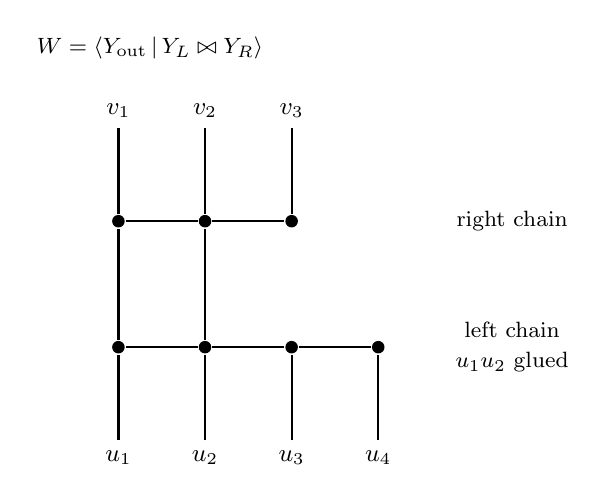
\begin{tikzpicture}[thick, every node/.style={font=\small}]
  % the left chain
  \foreach \i/\x in {1/0,2/1.1,3/2.2,4/3.3} {
    \node[circle, fill, inner sep=1.6pt] (L\i) at (\x,1.4) {};
  }
  \node (lA) at (0,0) {$u_1$};
  \node (lB) at (1.1,0) {$u_2$};
  \node (lC) at (2.2,0) {$u_3$};
  \node (lD) at (3.3,0) {$u_4$};
  \draw (lA) -- (L1); \draw (lB) -- (L2); \draw (lC) -- (L3); \draw (lD) -- (L4);
  \draw (L1) -- (L2); \draw (L2) -- (L3); \draw (L3) -- (L4);
  % the right chain, glued on the first two legs
  \foreach \i/\x in {1/0.0,2/1.1,3/2.2} {
    \node[circle, fill, inner sep=1.6pt] (R\i) at (\x,3.0) {};
  }
  \node (rA) at (0.0,4.4) {$v_1$};
  \node (rB) at (1.1,4.4) {$v_2$};
  \node (rC) at (2.2,4.4) {$v_3$};
  \draw (rA) -- (R1); \draw (rB) -- (R2); \draw (rC) -- (R3);
  \draw (R1) -- (R2); \draw (R2) -- (R3);
  \draw (L1) -- (R1); \draw (L2) -- (R2);
  \node[align=center] at (5.0,1.4) {\footnotesize left chain\\ \footnotesize $u_1u_2$ glued};
  \node[align=center] at (5.0,3.0) {\footnotesize right chain};
  \node[align=left] at (0.4,5.2)
    {\footnotesize $W=\langle Y_{\mathrm{out}}\,|\,Y_L\bowtie Y_R\rangle$};
\end{tikzpicture}
